\documentclass{beamer}

\usepackage[utf8]{inputenc}
\usepackage{hyperref}

\usetheme{Berkeley}
\beamertemplatenavigationsymbolsempty
\setbeamertemplate{headline}{}
 
\title{Erfassen von Daten in FoodChain-Lab 2}
\date{}
 
\begin{document}
\maketitle

\section{ }

\subsection{Aufgaben}
\begin{frame}
	\begin{itemize}
		\item In diesem Teil des Tutorials werden wir ein Rückwärts- and Vorwärts-Tracing für "Frozen Fruit Sales" ausführen.
		\item Sie müssen entweder erst Teil 1 des Tutorials bearbeiten oder folgende Dateien in eine leere Datenbank importieren, bevor sie mit diesem Teil des Tutorials starten.
		\item Start Template: \url{https://github.com/SiLeBAT/BfROpenLabResources/raw/master/GitHubPages/documents/Start_Tracing_Caterers.xlsx}
		\item Caterer 1 Template: \url{https://github.com/SiLeBAT/BfROpenLabResources/raw/master/GitHubPages/documents/Backtrace_request_Caterer 1.xlsx}
		\item Caterer 2 Template: \url{https://github.com/SiLeBAT/BfROpenLabResources/raw/master/GitHubPages/documents/Backtrace_request_Caterer 2.xlsx}
	\end{itemize}
\end{frame}
 
\subsection{1}
\begin{frame}
	\begin{center}
  		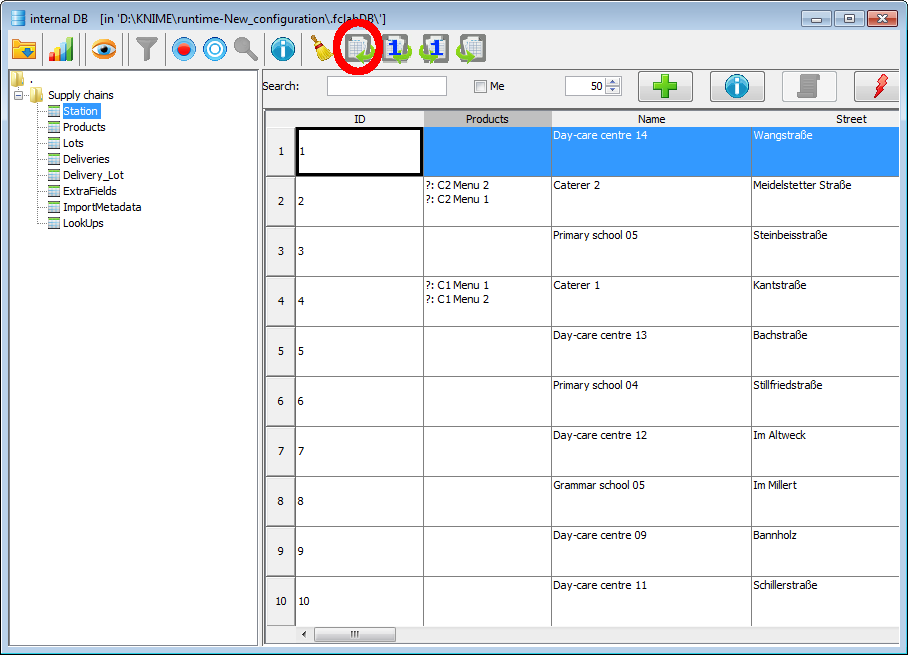
\includegraphics[height=0.6\textheight]{1.png}
	\end{center}
	\begin{itemize}
		\item Sie sollten das Datenbank-Fenster geöffnet haben.
		\item Drücken Sie den Button zum Generieren von Ruckwärts-Templates (roter Kreis).
	\end{itemize}
\end{frame}

\subsection{2}
\begin{frame}
	\begin{center}
  		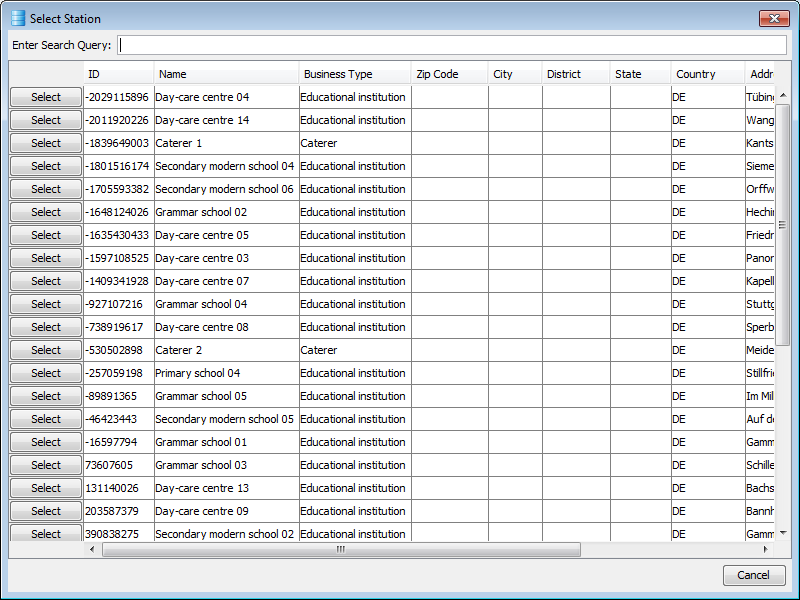
\includegraphics[width=0.4\textwidth]{2.png}
	\end{center}
	\begin{itemize}
		\item Da wir ein Rückwärts-Tracing für den Lieferanten (Supplier) "Frozen Fruit Sales" durchführen wollen, wählen Sie nur \textbf{Supplier} und klicken sie auf \textbf{OK}.
	\end{itemize}
\end{frame}

\subsection{3}
\begin{frame}
	\begin{center}
  		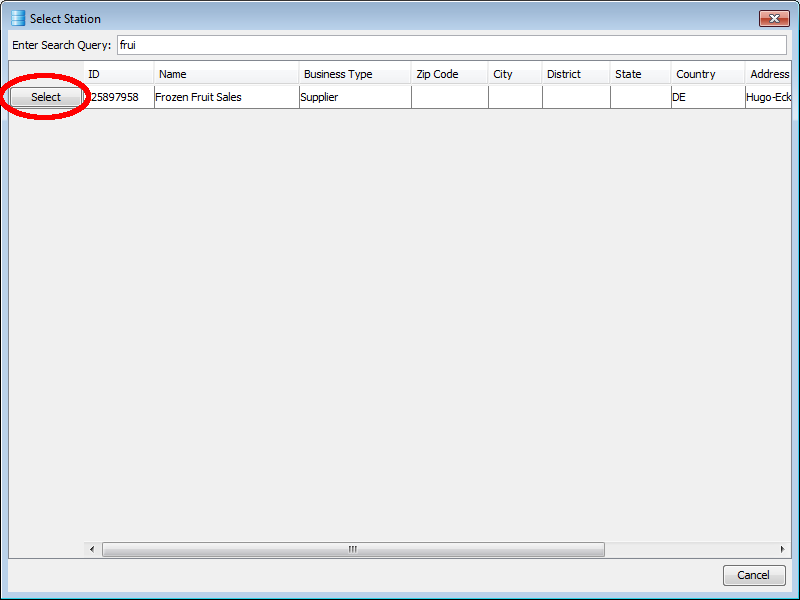
\includegraphics[height=0.5\textheight]{3.png}
	\end{center}
	\begin{itemize}
		\item In dem Dateidialog, der erscheint, können Sie den Ordner auswählen, in dem die generierten Templates gespeichert werden sollen.
		\item Wählen oder erzeugen Sie den gewünschten Ordner und klicken Sie auf \textbf{Save}.		
	\end{itemize}
\end{frame}

\subsection{4}
\begin{frame}
	\begin{center}
  		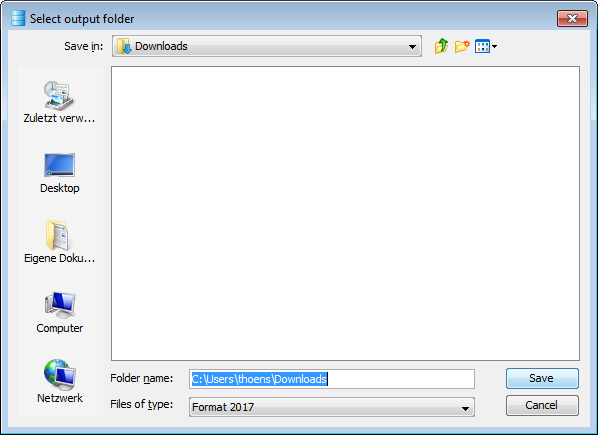
\includegraphics[width=0.8\textwidth]{4.png}
	\end{center}
	\begin{itemize}
		\item Sie werden benachrichtigt, dass ein Template generiert wurden.
		\item Klicken Sie auf \textbf{OK}.
	\end{itemize}
\end{frame}

\subsection{5}
\begin{frame}
	\begin{center}
  		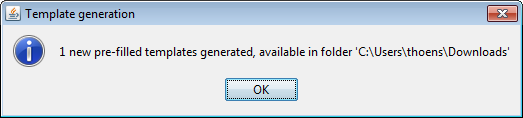
\includegraphics[width=0.95\textwidth]{5.png}
	\end{center}
	\begin{itemize}
		\item Öffnen Sie das generierte Template "Backtrace\_request\_Frozen Fruit Sales.xlsx".
		\item Fügen Sie die Stationen vom Screenshot zum \textbf{Stations}-Blatt hinzu.
		\item Diese Stationen beinhalten 3 Erdbeer-Lieferanten, die Erdbeeren an "Frozen Fruit Sales" geliefert haben, und einen Caterer, der Erdbeeren bekommen hat.
	\end{itemize}
\end{frame}

\subsection{6}
\begin{frame}
	\begin{center}
  		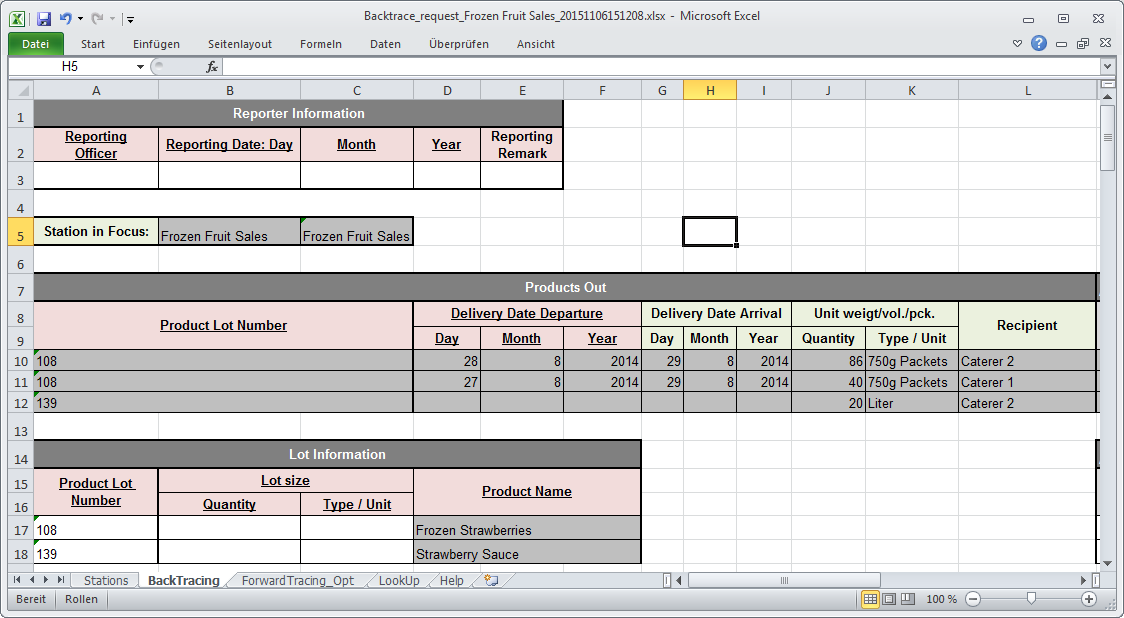
\includegraphics[width=0.95\textwidth]{6.png}
	\end{center}
	\begin{itemize}
		\item Im \textbf{BackTracing}-Blatt können Sie die drei ausgehenden Lieferungen von "Frozen Fruit Sales" sehen.
		\item Diese Lieferungen gehören zu den Lots "108" und "139".
	\end{itemize}
\end{frame}

\subsection{7}
\begin{frame}
	\begin{center}
  		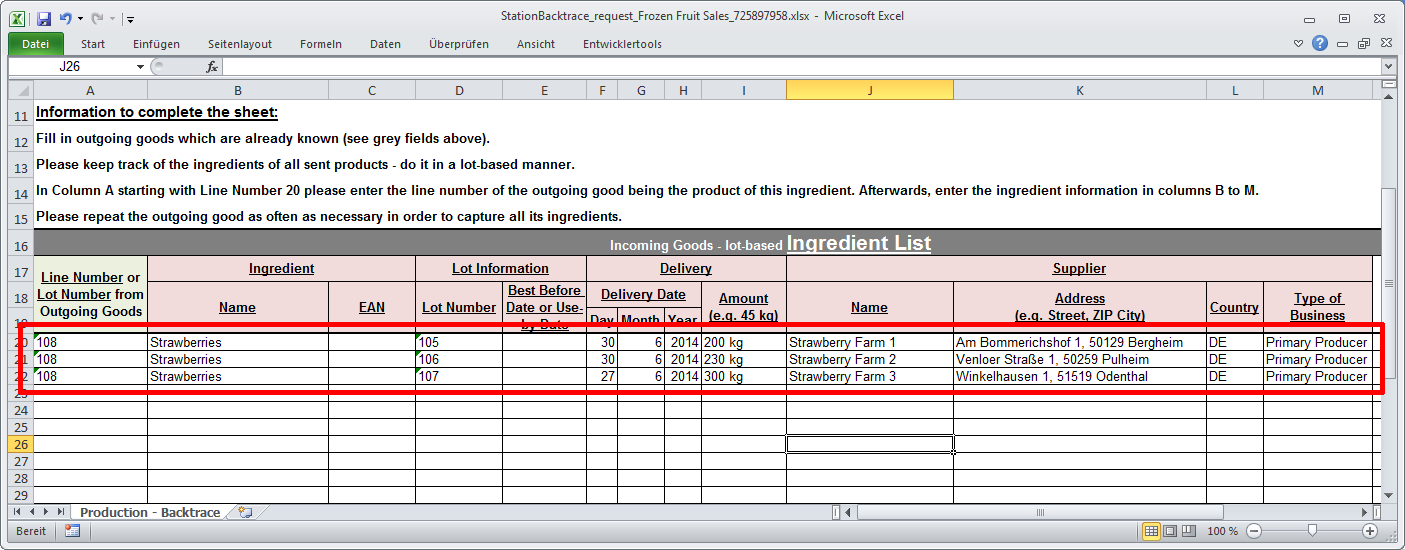
\includegraphics[width=0.95\textwidth]{7.png}
	\end{center}
	\begin{itemize}
		\item Nun scrollen Sie zu dem \textbf{Ingredients for Lot(s)}-Bereich.
		\item Tragen Sie die drei Lieferungen, welche als Zutaten für Lot "108" benutzt wurden, ein (siehe Screenshot).
	\end{itemize}
\end{frame}

\subsection{8}
\begin{frame}
	\begin{center}
  		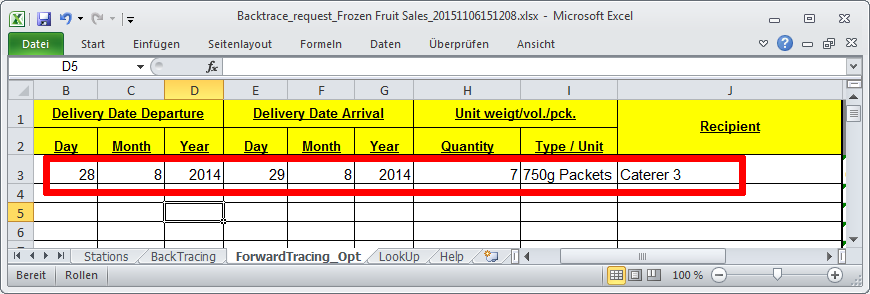
\includegraphics[width=0.95\textwidth]{8.png}
	\end{center}
	\begin{itemize}
		\item Lot "108" wurde nicht nur an "Caterer 1" und "Caterer 2" geliefert, sondern auch an einen dritten Caterer.
		\item Wir können diese Information im \textbf{ForwardTracing\_Opt}-Blatt eintragen.
		\item Tragen Sie die Lieferung an "Caterer 3" ein (siehe Screenshot).
		\item Speichern Sie das Dokument ("Backtrace\_request\_Frozen Fruit Sales.xlsx").
	\end{itemize}
\end{frame}

\subsection{9}
\begin{frame}
	\begin{center}
  		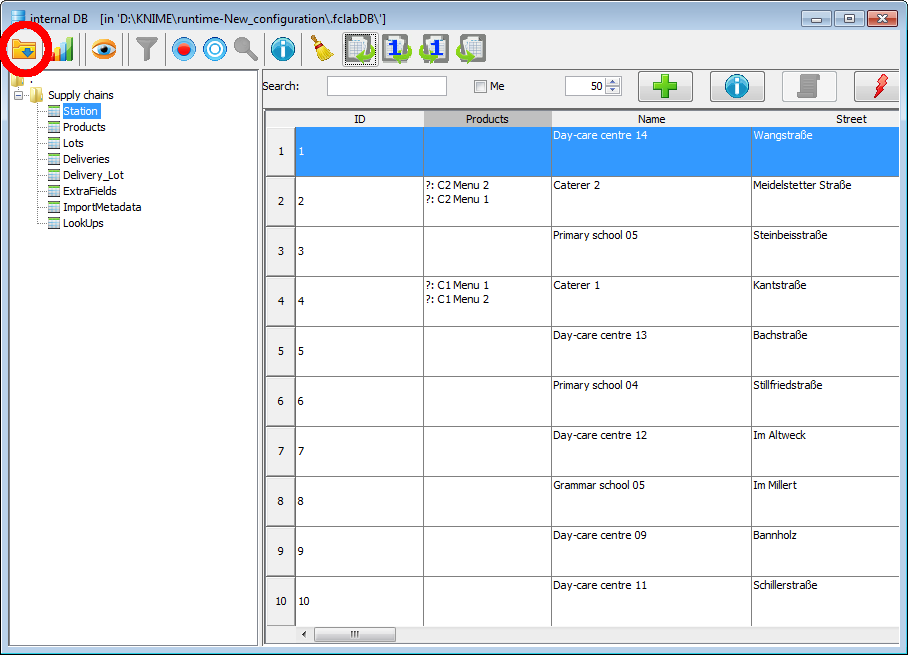
\includegraphics[height=0.6\textheight]{9.png}
	\end{center}
	\begin{itemize}
		\item Um das Dokument zu importieren, klicken Sie auf den Button \textbf{Table import} in der linken oberen Ecke des Datenbank-Fensters.
	\end{itemize}
\end{frame}

\subsection{10}
\begin{frame}
	\begin{center}
  		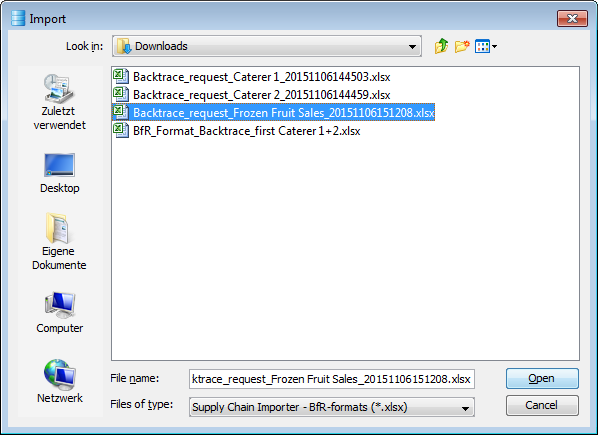
\includegraphics[height=0.5\textheight]{10.png}
	\end{center}
	\begin{itemize}
		\item Im Dateidialog, der erscheint, wählen Sie "Backtrace\_request\_Frozen Fruit Sales.xlsx" und klicken Sie auf \textbf{Open}.
	\end{itemize}
\end{frame}

\subsection{11}
\begin{frame}
	\begin{center}
  		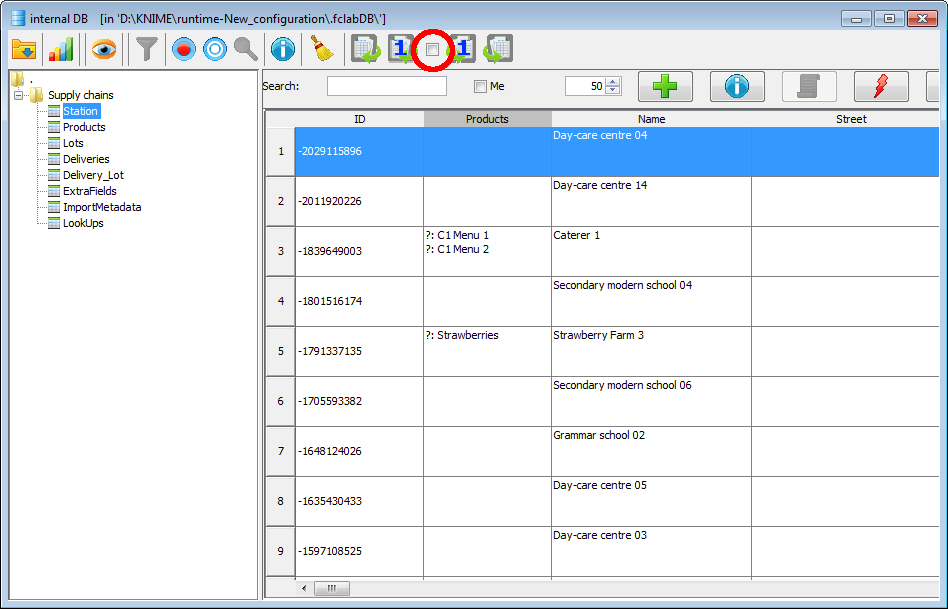
\includegraphics[width=0.7\textwidth]{11.png}
	\end{center}
	\begin{itemize}
		\item Sie werden benachrichtigt, dass es Warnungen beim Import gab.
		\item Klicken Sie auf \textbf{Show Details} um sich diese Warnungen anzuschauen.
	\end{itemize}
\end{frame}

\subsection{12}
\begin{frame}
	\begin{center}
  		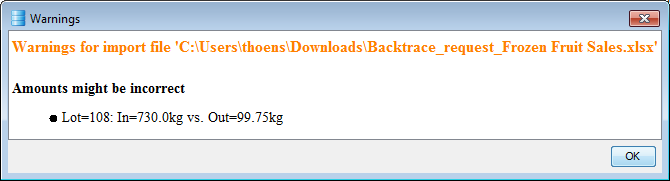
\includegraphics[width=0.95\textwidth]{12.png}
	\end{center}
	\begin{itemize}
		\item 730kg Erdbeeren sind in Lot "108" gegangen, aber alle Lieferungen von gefrorenen Erdbeeren aus Lot "108" summieren sich nur zu 99,75kg.
		\item Warnungen wie diese, sollen helfen Fehler in den importierten Daten zu finden.
		\item Diesmal ignorieren wir die Warnung einfach mal. Klicken Sie auf \textbf{OK}.
	\end{itemize}
\end{frame}

\subsection{13}
\begin{frame}
	\begin{center}
  		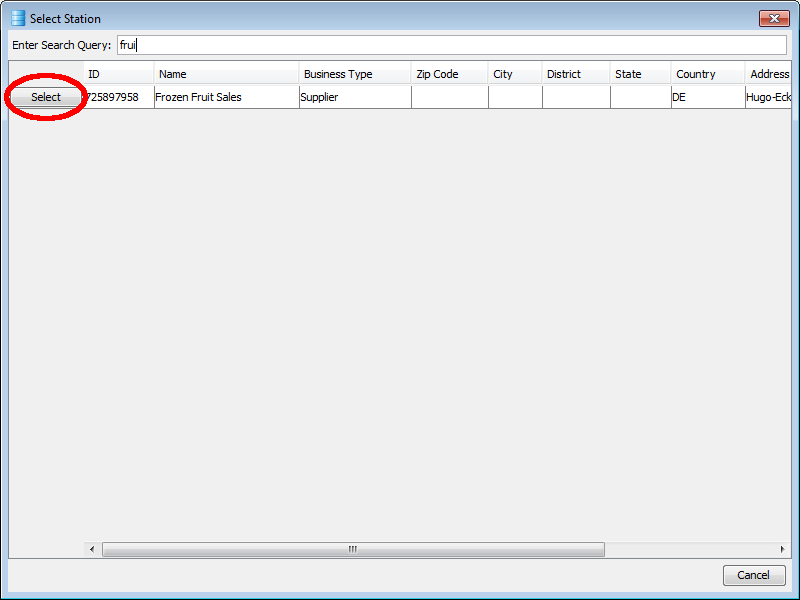
\includegraphics[height=0.6\textheight]{13.png}
	\end{center}
	\begin{itemize}
		\item We now know that lot "108" was also delivered to "Caterer 3" and we have imported this delivery into the database.
		\item Let's do a forward tracing from "Caterer 3".
		\item Press the button for generating the forward template for a specific station marked by the red circle.
	\end{itemize}
\end{frame}

\subsection{14}
\begin{frame}
	\begin{center}
  		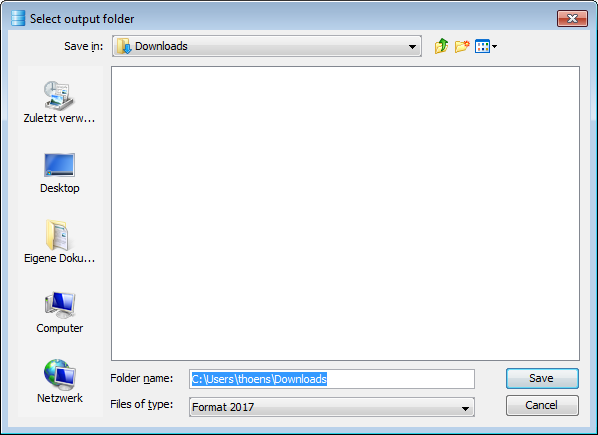
\includegraphics[width=0.95\textwidth]{14.png}
	\end{center}
	\begin{itemize}
		\item In the dialog that appears, you must select the station for which the template should be generated.
		\item Enter "cate" in the field after \textbf{Enter Search Query} and you will see that the table below only shows the caterers now.
		\item Press the \textbf{Select} button for "Caterer 3".
	\end{itemize}
\end{frame}

\subsection{15}
\begin{frame}
	\begin{center}
  		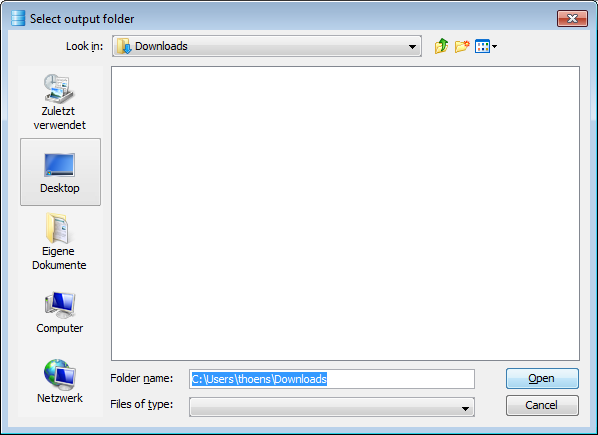
\includegraphics[height=0.5\textheight]{15.png}
	\end{center}
	\begin{itemize}
		\item In the file dialog that appears, you can specify the folder where the generated templates should be saved.
		\item Select the desired folder and press \textbf{Save}.
	\end{itemize}
\end{frame}

\subsection{16}
\begin{frame}
	\begin{center}
  		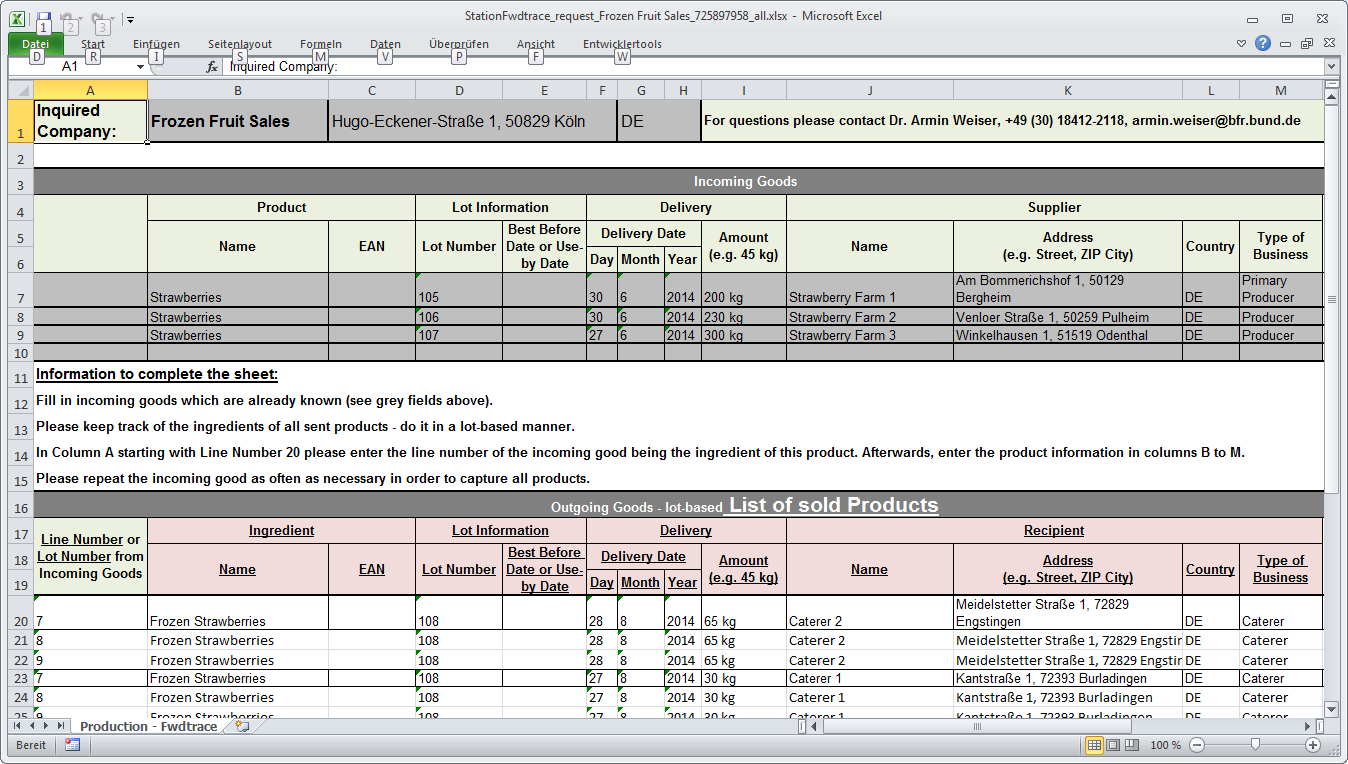
\includegraphics[width=0.8\textwidth]{16.png}
	\end{center}
	\begin{itemize}
		\item You'll be noticed, that one template was generated in the folder you specified.
		\item Press \textbf{OK}.
	\end{itemize}
\end{frame}

\subsection{17}
\begin{frame}
	\begin{center}
  		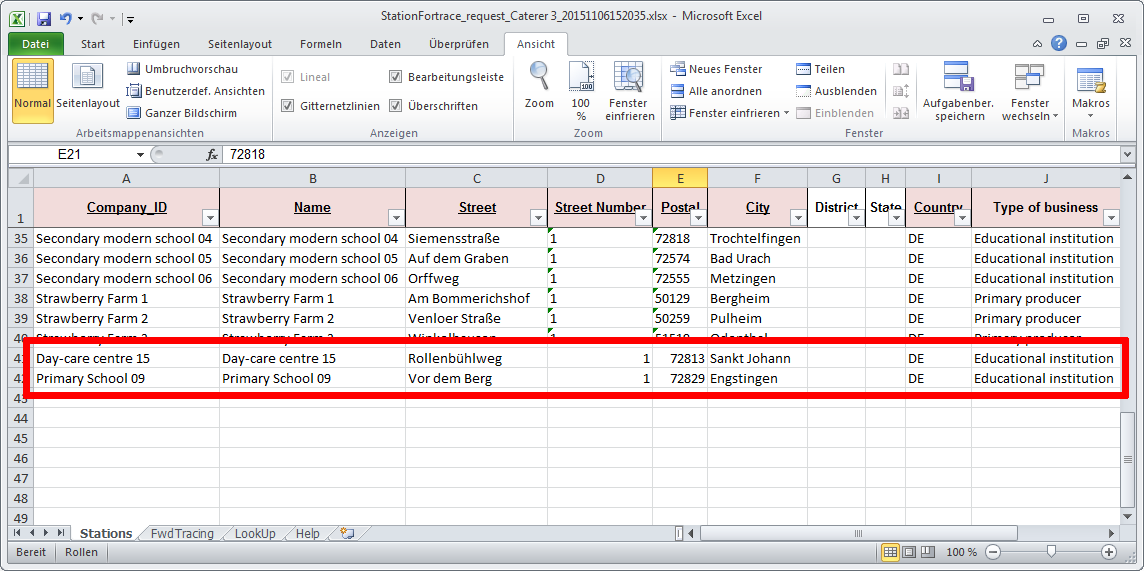
\includegraphics[width=0.95\textwidth]{17.png}
	\end{center}
	\begin{itemize}
		\item Open "StationFwdtrace\_request\_Caterer 3.xlsx".
		\item Enter the station from the screenshot in the \textbf{Stations} sheet.
	\end{itemize}
\end{frame}

\subsection{18}
\begin{frame}
	\begin{center}
  		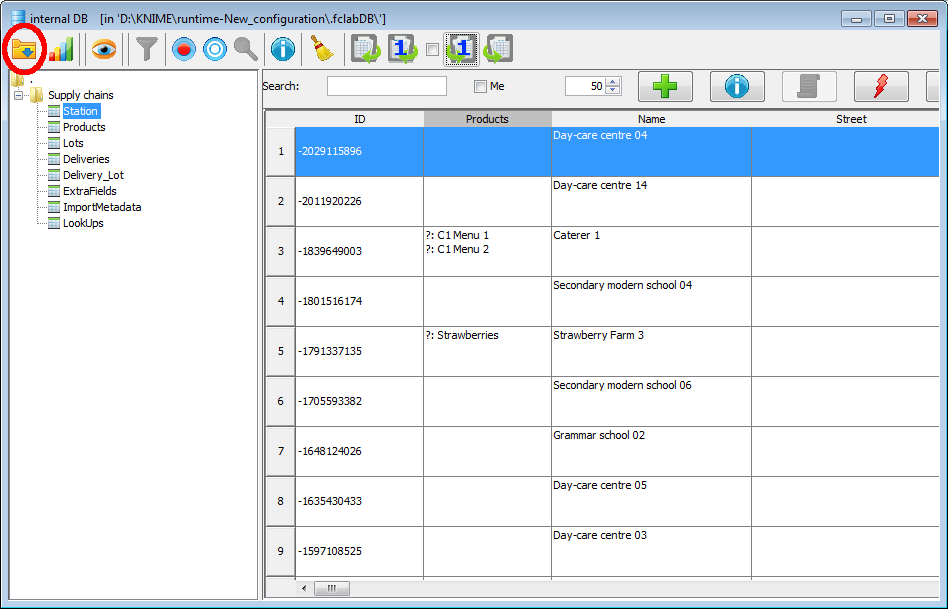
\includegraphics[width=0.9\textwidth]{18.png}
	\end{center}
	\begin{itemize}
		\item In the \textbf{FwdTracing} sheet you first have to enter all relevant outgoing lots of "Caterer 3". So add lot "C3M1" to the \textbf{Lot Information} section as shown on the screenshot (red rectangle).
		\item Now you can specify, that the delivery of "Frozen Strawberries" was used as an ingredient in this lot (red circle).
	\end{itemize}
\end{frame}

\subsection{19}
\begin{frame}
	\begin{center}
  		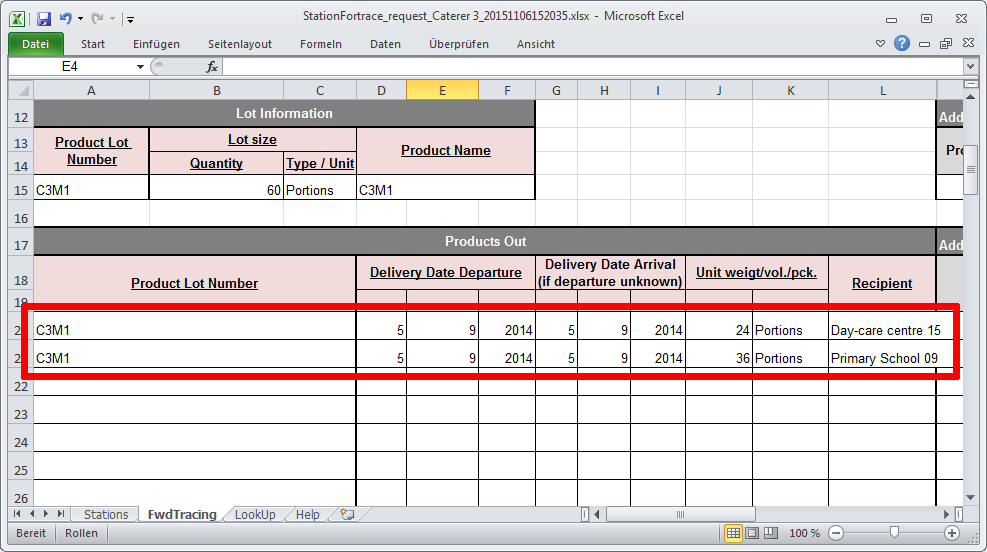
\includegraphics[width=0.95\textwidth]{19.png}
	\end{center}
	\begin{itemize}
		\item Scroll down to the \textbf{Products Out} section to specify the outgoing deliveries from lot "C3M1".
		\item Add the deliveries as shown on the screenshot.
		\item Save the completed document ("StationFwdtrace\_request\_Caterer 3.xlsx").
	\end{itemize}
\end{frame}

\subsection{20}
\begin{frame}
	\begin{center}
  		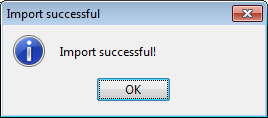
\includegraphics[height=0.6\textheight]{20.png}
	\end{center}
	\begin{itemize}
		\item To import this file click on the \textbf{Table import} button in the upper left corner of the database interface.
	\end{itemize}
\end{frame}

\subsection{21}
\begin{frame}
	\begin{center}
  		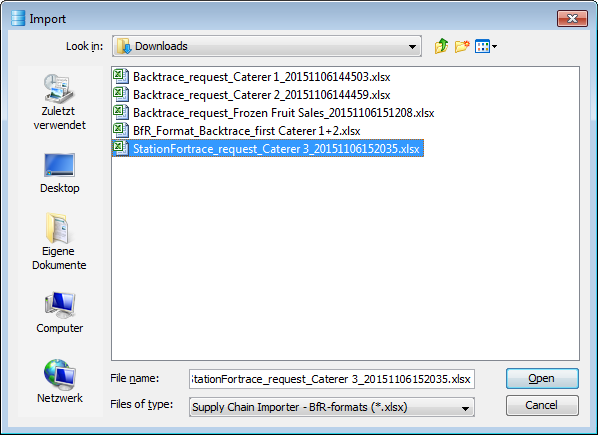
\includegraphics[height=0.5\textheight]{21.png}
	\end{center}
	\begin{itemize}
		\item In the file dialog that appears, select "StationFwdtrace\_request\_Caterer 3.xlsx" and press \textbf{Open}.
	\end{itemize}
\end{frame}

\subsection{22}
\begin{frame}
	\begin{center}
  		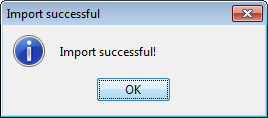
\includegraphics[width=0.4\textwidth]{22.png}
	\end{center}
	\begin{itemize}
		\item You'll see a message that the import was successful.
		\item Press \textbf{OK}.
	\end{itemize}
\end{frame}

\end{document}